\subsection{Introduction}
Ce projet est un projet réalisé dans le cadre d'un PFA (Projets au fil de l'année)
de l'école ENSEIRB-MATMECA de Talence durant l'année scolaire 2023/2024. \\
\newline
Il vise à développer une application informatique permettant d’inciter chaque adhérent
et chaque structure à limiter son impact sur le climat, notamment en mesurant les 
progrès réalisés au travers de différentes actions. \\L'application sera élaborée en prenant en compte l'expérience et les besoins spécifiques des Scouts et Guides de France. Toutefois, sa conception la rendra accessible à toute structure souhaitant s'engager dans une démarche similaire en faveur de la réduction de son empreinte écologique. L'application sera accessible via une interface web conviviale, facilitant ainsi l'utilisation sur divers appareils. 
\\
\newline
Le projet EcoScout est disponible sur GitHub, accessible à l'adresse suivante :
\begin{center}
    \url{https://github.com/tloloum/EcoScout}
\end{center}
Le code source du projet EcoScout est publié en tant que logiciel open source, 
ce qui signifie que le code est librement accessible et modifiable par la communauté. 


\subsection{Définition des termes du projet}

Différents termes importants seront utilisés lors de la réalisation de ce projet, en voici une liste non exhaustive.
\begin{itemize}
    \item \textbf{Utilisateur} : Une personne qui utilise l'application
    \item \textbf{Structure} : Un utilisateur moral utilisant l'application
    \item \textbf{Responsable:} Utilisateur responsable d'une structure donnée.
    \item \textbf{Événement:} Événement planifié avec une durée définie organisé par une structure.
    \item \textbf{Défi:} Jeu invitant des structures à atteindre un ou plusieurs objectifs dans un temps donné (qui peut être lié à un événement ou une structure ou un utilisateur).
    \item \textbf{Objectif:} Défini par une mesure (un élément qui peut se mesurer), une valeur (une donnée chiffrée ou référence) 
    et un critère (un opérateur de comparaison). 
\end{itemize}

Les \textbf{Défis} dans l'application EcoScout sont définis comme un ensemble d' \textbf{Objectifs} 
à atteindre dans un temps donné, avec des critères spécifiques. La \textbf{base d'objectifs} 
fournie dans l'application sert de point de départ, offrant une variété d'objectifs aux utilisateurs. 
Chaque \textbf{structure} a la capacité de créer ses propres objectifs. Les objectifs créés par une 
structure sont visibles par toutes les structures qui en dépendent, favorisant la transparence et la collaboration. 

\begin{tcolorbox}[colback=white!2,
    colframe=black!60,
    title=\textbf{Exemple de Défis}
   ]
   Le \textbf{Groupe de Chamarande} crée un défi appelé "Déplacements Carbonés" dont les objectifs spécifiques peuvent inclure la réduction des émissions de carbone 
   liées aux déplacements. Les structures dépendantes, comme \textbf{L'Unité Louveteaux-Jeannettes}, 
   participent activement à la réalisation de ces objectifs.
\end{tcolorbox}


\begin{tcolorbox}[colback=white!2,
    colframe=black!60,
    title=\textbf{Exemple d'utilisation}
   ]
   \textbf{Yanis Toirscout} est un utilisateur d'EcoScout. Il utilise l'application 
    pour gérer et suivre les activités de son groupe de Chamarande.\\
    \newline
    \textbf{Groupe Chamarande} représente la structure regroupant différentes 
    unités et membres. Ici \textbf{Yanis Toirscout} est le responsable du \textbf{Groupe Chamarande}.
    \textbf{L'unité Louveteaux-Jeannettes} est membre du \textbf{Groupe Chamarande}. 
    Par exemple on pourrait avoir Alice, fille de Yanis, qui fait partie de l'unité Louveteaux-Jeannettes.\\
    \newline
    Le \textbf{Week-end Déplacements Durables} peut être un événement organisé par le \textbf{Groupe Chamarande}.
    Il sera définie dans un délai prédéterminé, ici un weekend. Le \textbf{Défi} de cet événement pourrait être 
    d'inviter les différentes structures spécifique à limiter leur empreinte carbone a un certain nombre.
\end{tcolorbox}

\begin{figure}[h]
    \centering
    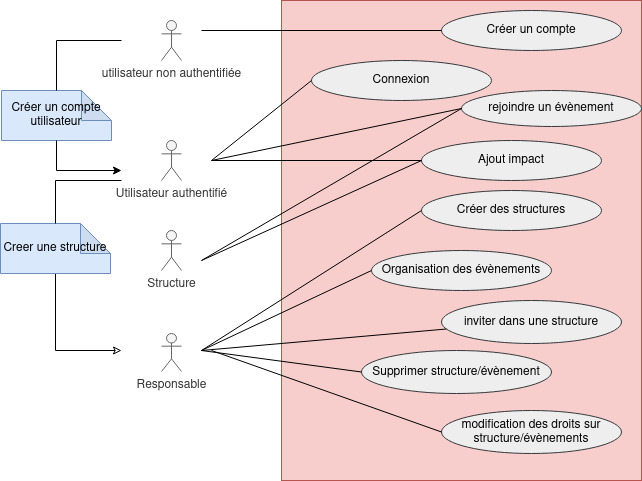
\includegraphics[width=0.8\linewidth]{pictures/use_case_pfa.jpg}
    \caption{Diagramme de cas d'utilisation}
    \label{fig:diag_use_case}
\end{figure}




\subsection{Règles définies}
Différentes règles ont été définies par rapport à l'interaction des différents éléments du projet.
\begin{itemize}
    \item Une structure a entre 1 et n responsables.
    \item Un utilisateur est responsable de sa structure "personne physique".
    \item Un utilisateur peut être responsable de 0 à n structures.
\end{itemize}

\begin{figure}
    \centering
    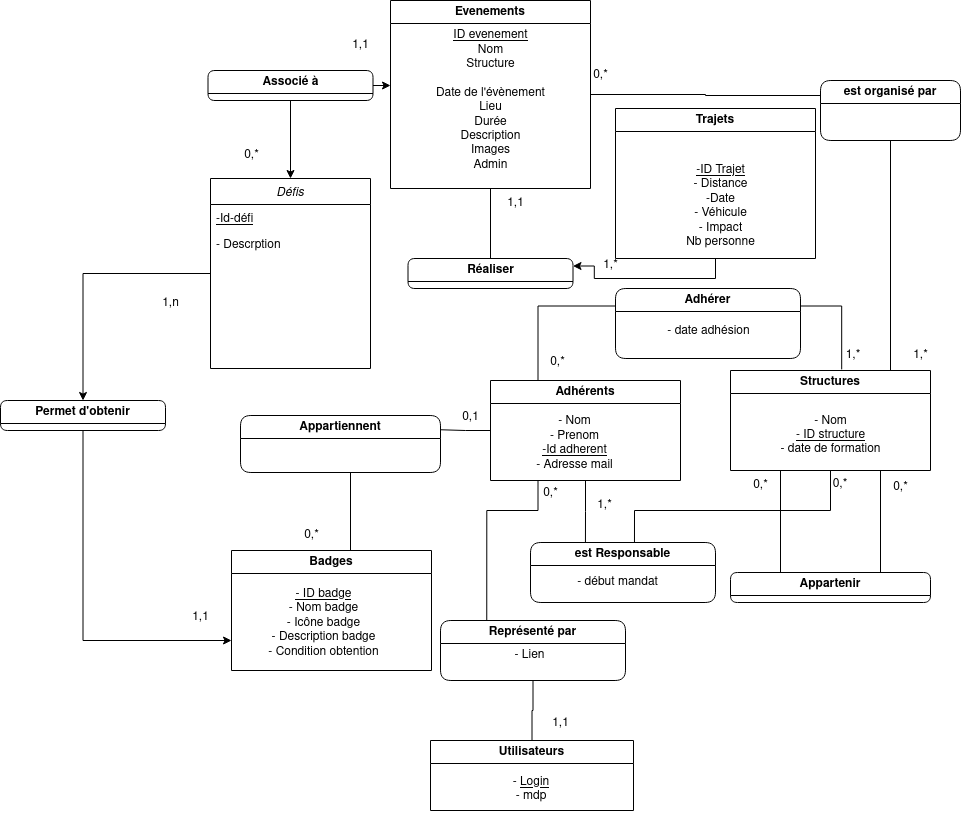
\includegraphics[width=1.1\linewidth]{pictures/Copie de Copie de CDC_PFA.drawio.png}
    \caption{Diagramme conceptuel}
    \label{fig:diag_concept}
\end{figure}

